\bigskip
\section{Equivalencia de nudos: movimientos de Reidemeister.}\label{seccion4}
Dos nudos K1 y K2 serán equivalentes (K1 $\thicksim$ K2) si podemos distorsionar uno de ellos en el otro sin hacer ningún corte. \\

Para ver si dos proyecciones corresponden a nudos equivalentes, usaremos el conepto de isotopía plana. Más precisamente, definimos una \textbf{isotopía plana} de las proyecciones P1 y P2 de nudos como la aplicación continua $F: \mathds{R}^{2}$ x $[0,1] \rightarrow \mathds{R}^{2}$ tal que $F_{0}=identidad$, $F_{1}(P1) = P2$ y $F_{t}$ es un homeomorfismo $\forall t$.\\

Los movimientos de Reidemeister que vamos a ver a continuación nos permiten cambiar la proyección de un nudo de modo que se cambie la relación entre los cruces pero que no cambie el nudo al que representa la proyección. \\
Cada uno de estos movimientos es una isotopía:\\

\textbf{Primer movimiento de Reidemeister - R1}\\
En cualquier zona de la proyección nos permite añadir o eliminar un giro tal y como vemos en la figura \ref{movi1}.
  \begin{figure}[h!]
  	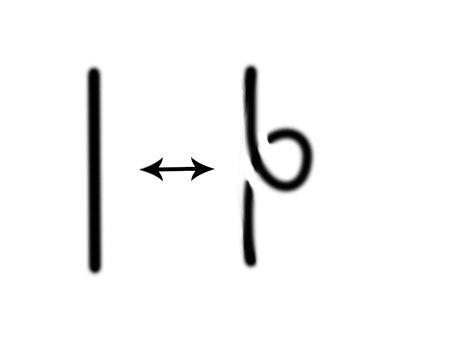
\includegraphics[width=5cm]{inudos/movi1.png}
  	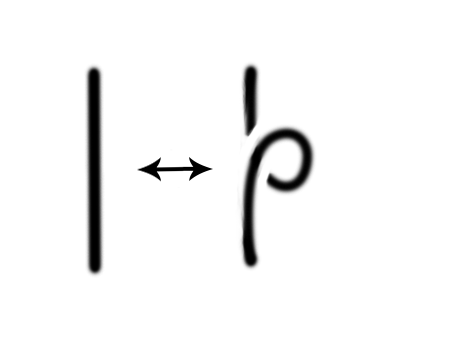
\includegraphics[width=5cm]{inudos/movi2.png}
  	\centering
  	\caption{Primer movimiento Reidemeister.}
  	\label{movi1} 
  \end{figure}
  
	\textbf{Segundo movimiento de Reidemeister - R2.}\\
Nos permite añadir o eliminar dos cruces del nudo como se ve en la figura \ref{movi2}.
    \begin{figure}[h!]
    	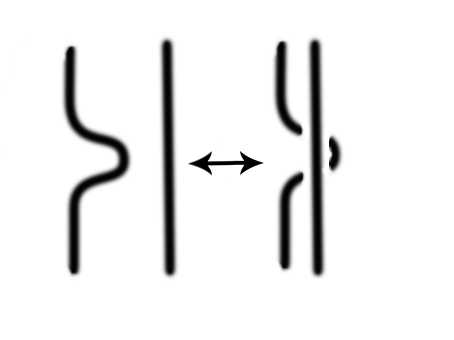
\includegraphics[width=7cm]{inudos/movi3.png}
    	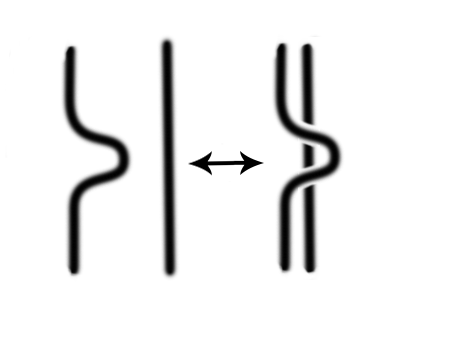
\includegraphics[width=7cm]{inudos/movi4.png}
    	\centering
    	\caption{Segundo movimiento de Reidemeister.}
    	\label{movi2} 
    \end{figure}
    
	\textbf{Tercer movimiento de Reidemeister - R3.}\\
Nos permite deslizar una hebra del nudo de un lado de un cruce al otro lado del cruce. Veamos la figura \ref{movi3} para aclarar la idea.
      \begin{figure}[h!]
      	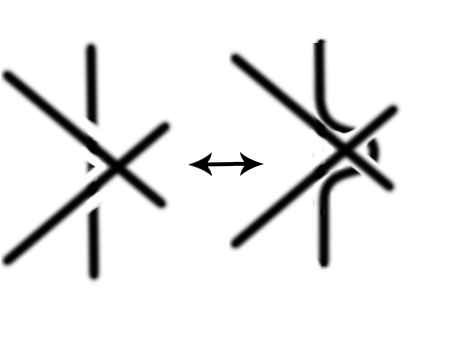
\includegraphics[width=7cm]{inudos/movi5.png}
      	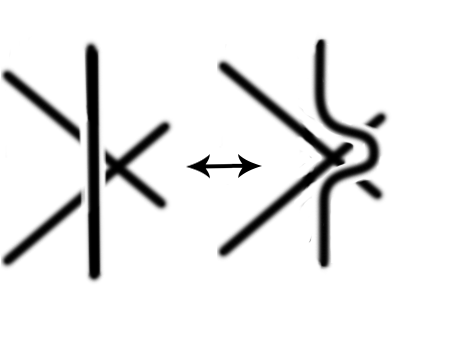
\includegraphics[width=7cm]{inudos/movi6.png}
      	\centering
      	\caption{Tercer movimiento de Reidemeister.}
      	\label{movi3} 
      \end{figure}
  

\begin{teo} \textbf{Teorema de Reidemeister.} Sean P1 y P2 las proyecciones que representan a dos nudos K1 y K2, respectivamente. Entonces, K1 $\thicksim$ K2 si, y solo si, P1 y P2 están conectados por una secuencia finita de movimientos de Reidemeister e isotopías planas.
\end{teo}

Veamos un ejemplo en el que vemos la equivalencia de dos proyecciones, que en un primer momento podrían no parecernos equivalentes:
  \begin{figure}[h!]
  	\subfigure[P1]{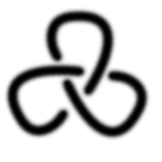
\includegraphics[width=3cm]{inudos/3f.png}}
  	\subfigure[R1]{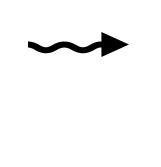
\includegraphics[width=2cm]{inudos/flecha.png}}
  	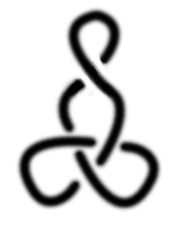
\includegraphics[width=3cm]{inudos/3fseg.png}
  	\subfigure[R3]{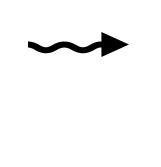
\includegraphics[width=2cm]{inudos/flecha.png}}
  	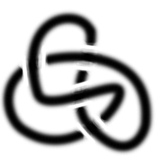
\includegraphics[width=3cm]{inudos/fase3.png}
  	\subfigure[Isotopia]{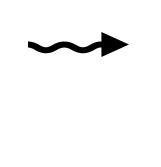
\includegraphics[width=2cm]{inudos/flecha.png}}
  	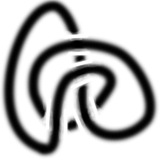
\includegraphics[width=3cm]{inudos/fase4.png}
  	\subfigure[R3]{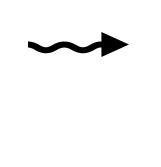
\includegraphics[width=2cm]{inudos/flecha.png}}
  	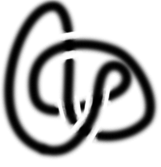
\includegraphics[width=3cm]{inudos/fase5.png}
  	\subfigure[R1]{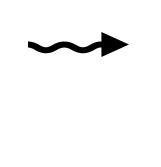
\includegraphics[width=2cm]{inudos/flecha.png}}
  	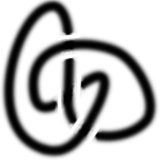
\includegraphics[width=3cm]{inudos/fase6.png}
  	\subfigure[Isotopia]{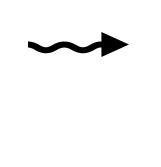
\includegraphics[width=2cm]{inudos/flecha.png}}
  	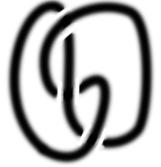
\includegraphics[width=3cm]{inudos/fase7.png}
  	\subfigure[Isotopia]{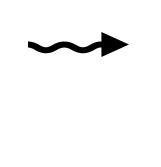
\includegraphics[width=2cm]{inudos/flecha.png}}
  	\subfigure[P2]{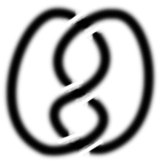
\includegraphics[width=3cm]{inudos/fase8.png}}
  	\centering
  	\caption{Equivalencia de dos proyecciones de nudos.}
  	\label{algosj} 
  \end{figure}

Gracias a dicho teorema podremos estudiar si dos proyecciones representan el mismo nudo. Para ello tendremos que encontrar una secuencia de movimientos de Reidemeister que nos lleve de una proyección a la otra. Sin embargo, este proceso puede no tener el número de movimientos intermedios limitado por lo que no tiene mucho sentido implementarlo.\\
 
 Aunque este teorema no nos permita ver de una forma cómoda la equivalencia entre dos nudos en la práctica (por la fuerte complejidad) si que nos permite obtener una conclusión esencial:\\
 
 Si una propiedad de un nudo no cambia al aplicarle cualquiera de estos tres movimientos de Reidemeister, entonces esta propiedad no va a cambiar por muchas deformaciones que se le hagan al nudo. En definitiva, si un nudo cumple cierta propiedad y otro nudo no la cumple, esos nudos no podrán ser equivalentes. Incidiremos en esta idea en la siguiente Sección \ref{seccion5}.
 